\chapter{Hlavní funkce aplikace Dayplanner}  
\hspace{14pt} Tato kapitola stručně popisuje hlavní funkce, které uživatel může v aplikaci využívat.  

\section{Hlavní aktivita}  
\hspace{14pt} V hlavní aktivitě si uživatel může přidávat úkoly a návyky kliknutím na tlačítko „+“(\autoref{fig:main-acc} - Add button) se zobrazí přehledný dialog, ve kterém si může zvolit, zda chce přidat nový úkol nebo návyk. Poté, co uživatel klikne na jednu z možností, zobrazí se mu dialog na přidání(\autoref{fig:main-acc} - Add dialog). Když uživatel klikne na ikonu položky může ji i upravovat nebo smazat(\autoref{fig:main-acc} - Edit dialog).

\begin{figure}[H]
    \centering
    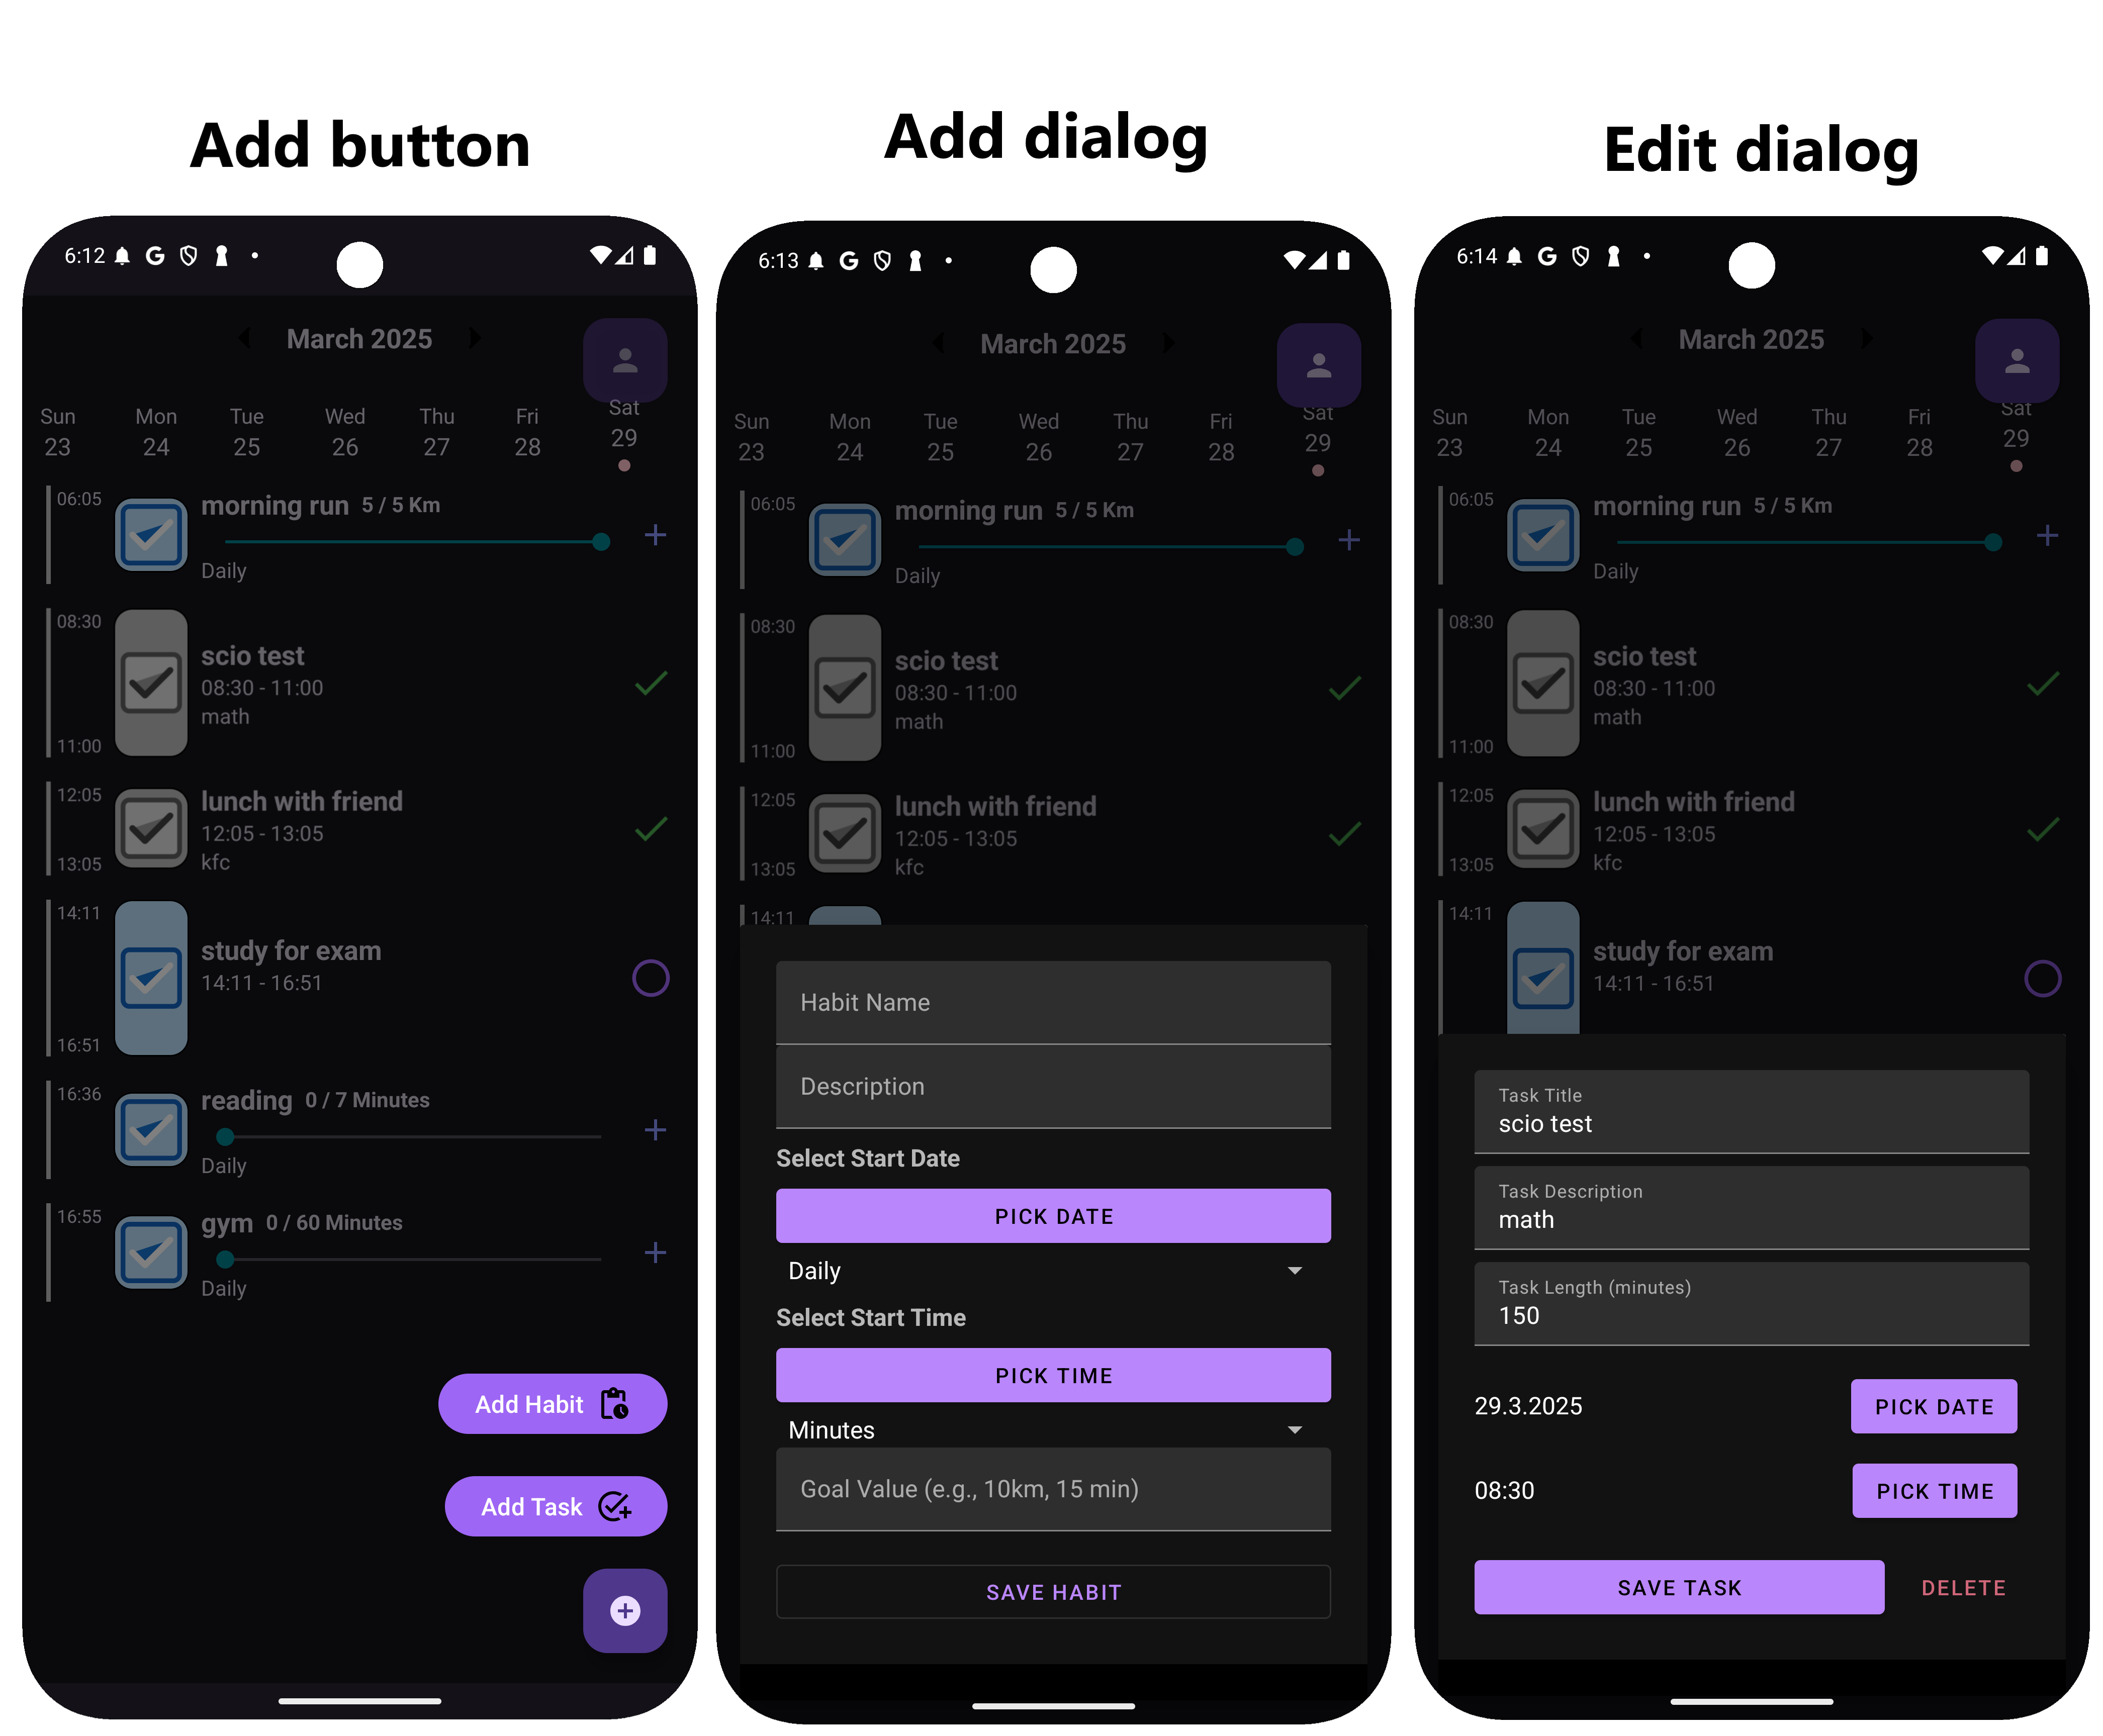
\includegraphics[width=1\linewidth]{images/nice.png}
    \caption{Main activity functions}
    \label{fig:main-acc}
\end{figure}

\newpage

Kalendář umožňuje přepínání mezi jednotlivými dny buď swipováním do stran, nebo výběrem konkrétního dne pomocí kalendáře(\autoref{fig:date-pickerl}). Po kliknutí na den se přesune časová osa na vybraný den a zobrazí relevantní data.  
\begin{figure}[H]
    \centering
    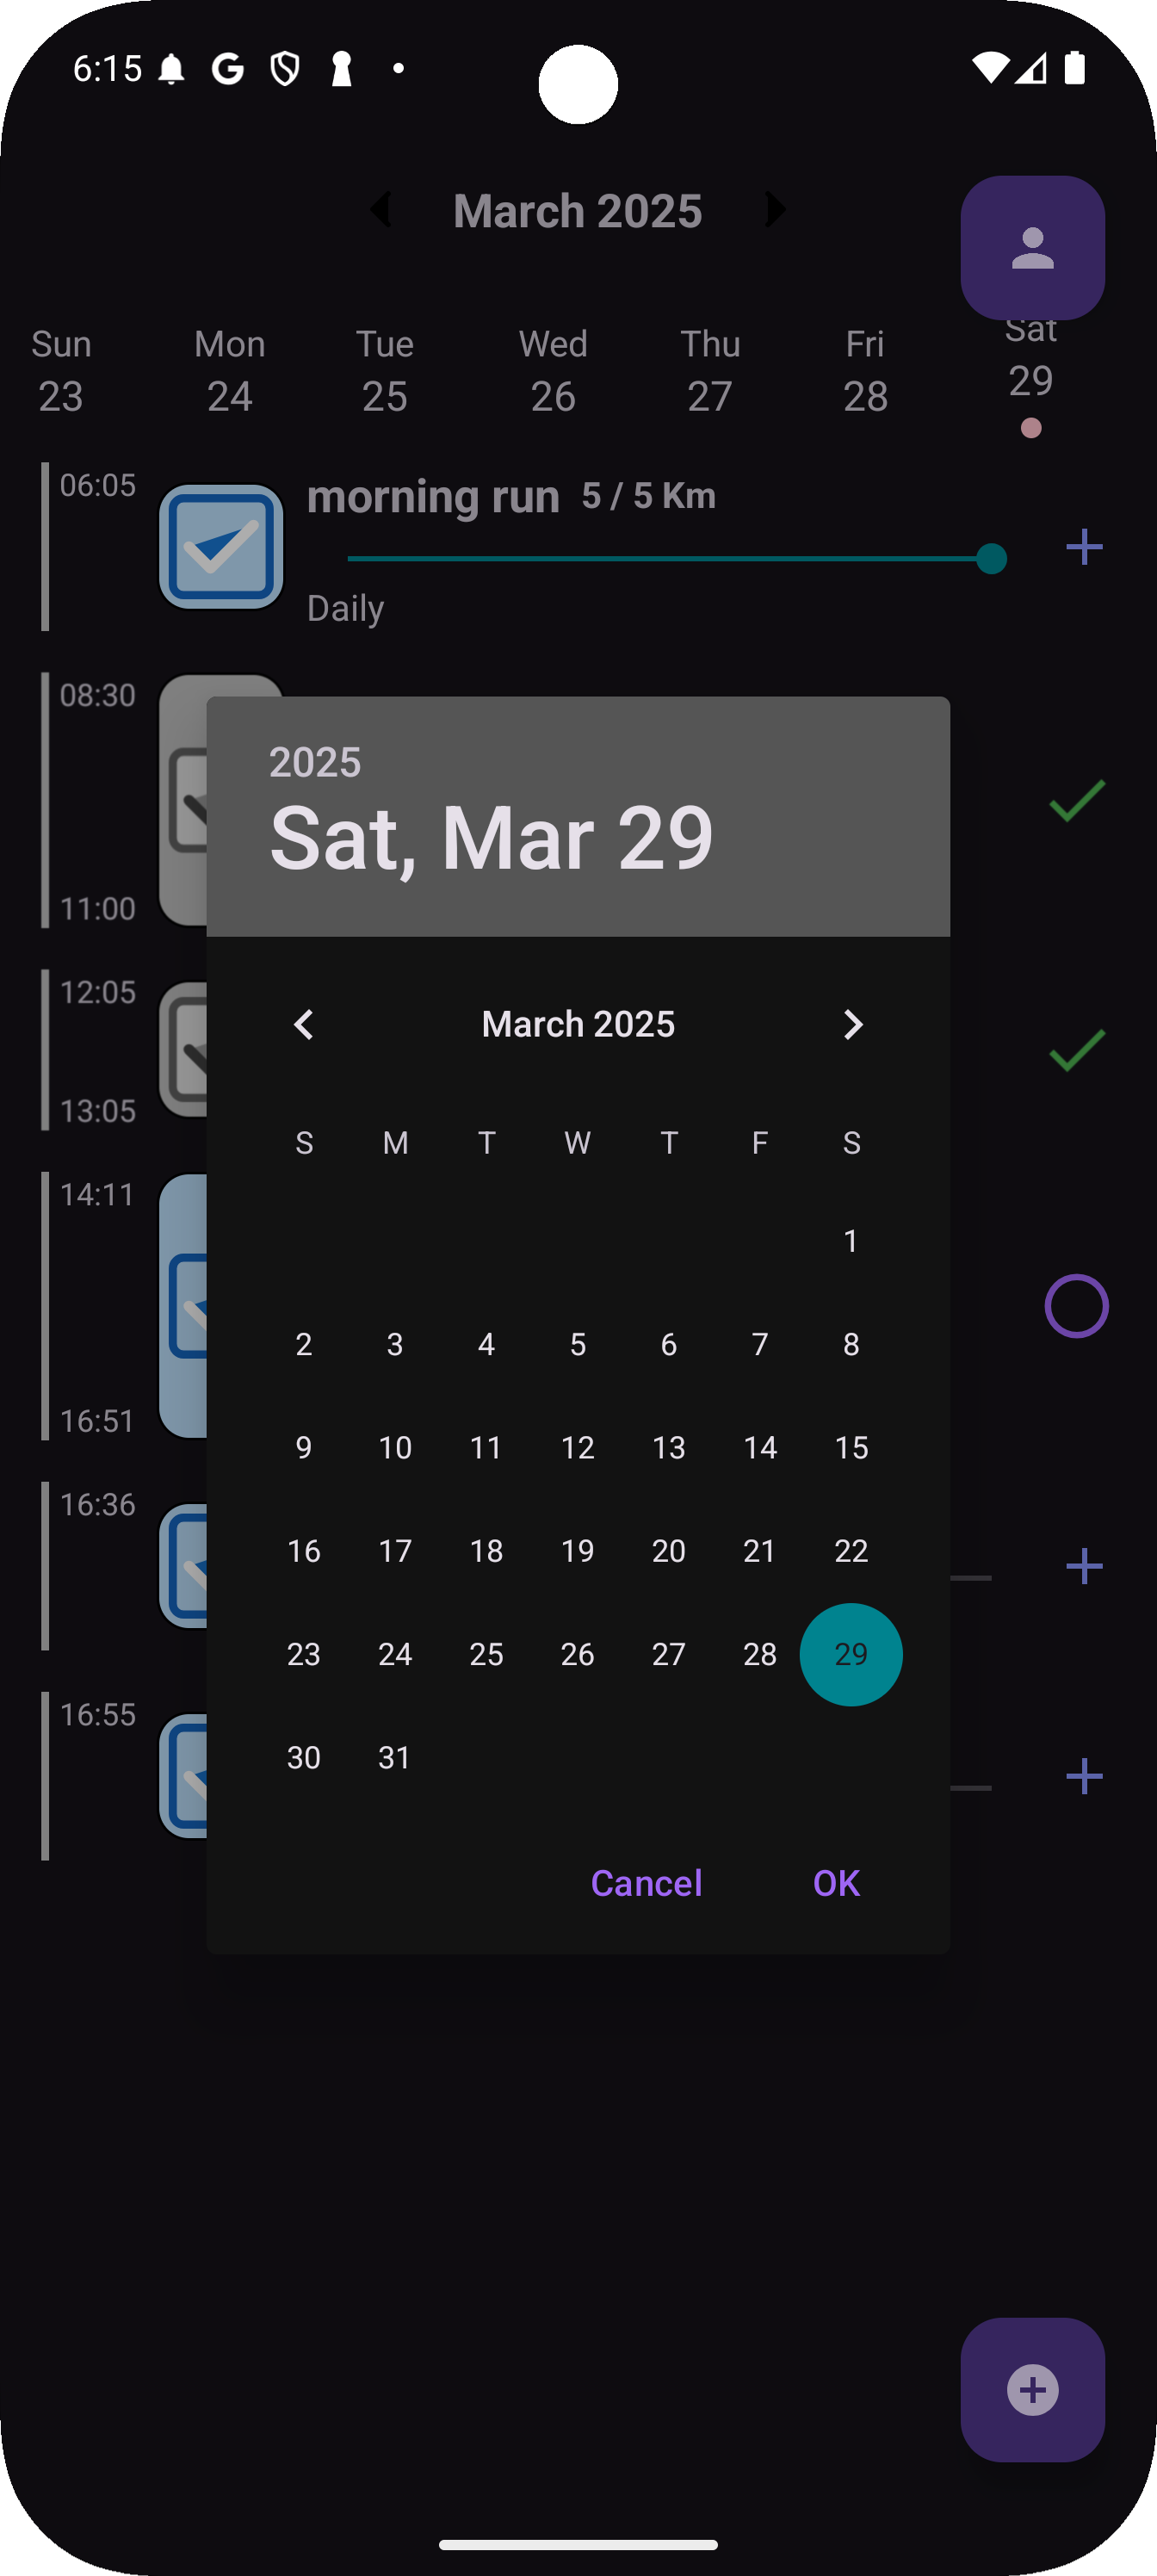
\includegraphics[width=0.3\linewidth]{images/kalendar.png}
    \caption{Kalendář}
    \label{fig:date-pickerl}
\end{figure}

\newpage

\section{Uživatelský profil}  
\hspace{14pt} V uživatelském profilu si může uživatel přizpůsobit vzhled aplikace změnou mezi světlým a tmavým režimem. Pokud je přihlášen pomocí emailu, má možnost změnit heslo, avšak tato funkce není dostupná pro uživatele přihlášené přes Google účet. Dále si může nastavit, zda chce dostávat notifikace, a povolit nebo zakázat upozornění podle svých preferencí. Níže můžeme vidět ukázku tmavého a světlého režimu.

\begin{figure}[H]
    \centering
    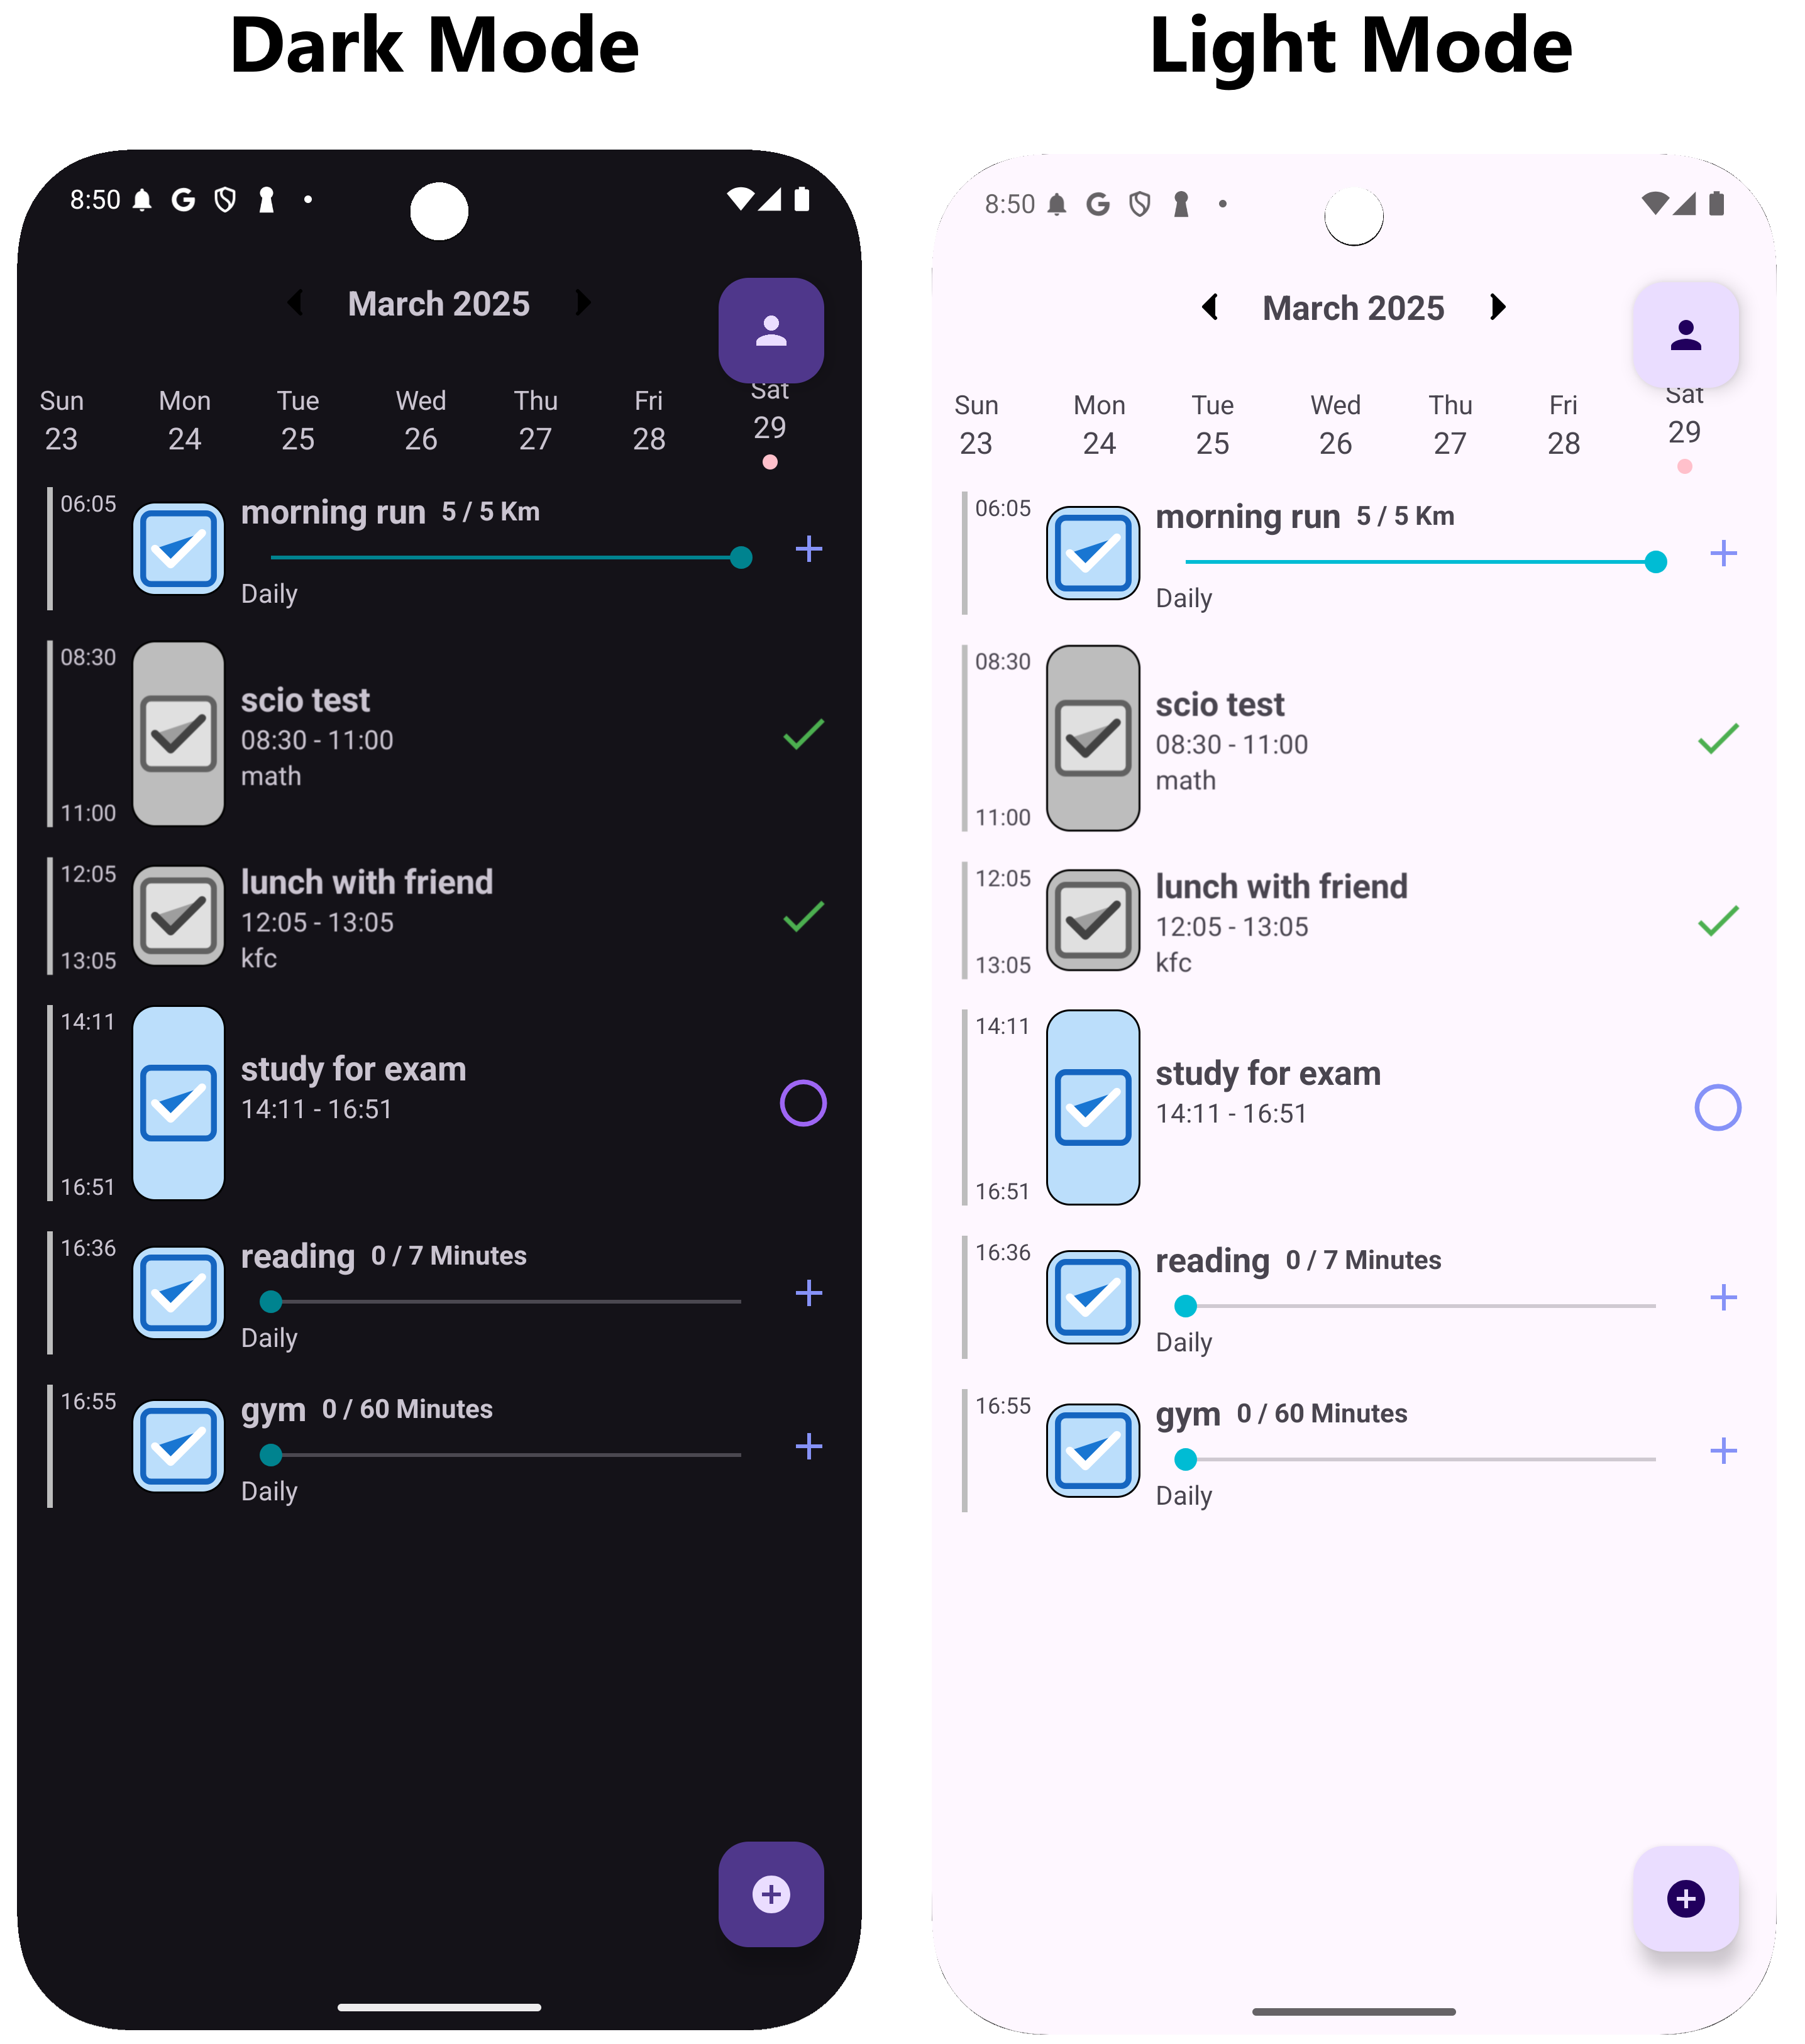
\includegraphics[width=0.7\linewidth]{images/lightdark.png}
    \caption{Dark and Light Mode}
    \label{fig:enter-label}
\end{figure}
\newpage

